\section{Experimental Results}
\label{sec:experimental_results}

This section evaluates KG-Hybrid through clean classification,
probabilistic calibration, controlled component comparisons, per-class
analysis, input perturbations, confidence-aware routing, and model
complexity. Results are separated by experimental protocol and model
configuration. In particular, the compact five-seed comparison is
distinguished from the completed noncompact cross-validation experiment,
the corrected saved-checkpoint evaluation, and earlier robustness
experiments. Measurements from these protocols are not treated as
interchangeable estimates of the same model.

% --------------------------------------------------------------------
\subsection{Experimental Setup}
% --------------------------------------------------------------------

\subsubsection{Dataset}

Experiments use the Crop Recommendation
dataset~\cite{cropdataset}, containing 2,200 records, seven numerical
input variables, and 22 crop classes. Each class contains 100 records.
The input variables are nitrogen, phosphorus, potassium, temperature,
humidity, pH, and rainfall.

Table~\ref{tab:dataset_stats} reports descriptive statistics recomputed
from the complete raw dataset. Values retain the numerical encoding
provided by the dataset. Physical concentration units are not assigned
to the nutrient variables because their measurement basis has not been
independently established.

\begin{table}[t]
\centering
\caption{Descriptive Statistics of the Raw Dataset.
Standard deviations use the sample estimator.}
\label{tab:dataset_stats}
\small
\begin{tabular}{lrrrr}
\hline
Feature & Mean & Std. & Min. & Max. \\
\hline
Nitrogen    & 50.55  & 36.92 & 0.00  & 140.00 \\
Phosphorus  & 53.36  & 32.99 & 5.00  & 145.00 \\
Potassium   & 48.15  & 50.65 & 5.00  & 205.00 \\
Temperature & 25.62  & 5.06  & 8.83  & 43.68  \\
Humidity    & 71.48  & 22.26 & 14.26 & 99.98  \\
pH          & 6.47   & 0.77  & 3.50  & 9.94   \\
Rainfall    & 103.46 & 54.96 & 20.21 & 298.56 \\
\hline
\end{tabular}
\end{table}

The experiments measure agreement with the benchmark crop labels.
They do not establish crop yield, profitability, or agronomic
suitability under field conditions.

\subsubsection{Evaluation Protocols}

The principal controlled comparison uses five seeds:
42, 123, 2024, 3407, and 9999. Each seed generates a separate
stratified 70\%/15\%/15\% training--validation--test partition,
containing 1,540, 330, and 330 records, respectively.
Thus, variability reflects both partition changes and stochastic
training, rather than random initialization alone.

Within each seed, all model variants use identical partition
identities. The hybrid variants additionally share the seed-specific
XGBoost booster, pretrained FT-Transformer backbone, leaf-embedding
initialization, and prediction-head initialization. Standardization
parameters are fitted exclusively on the training partition and applied
unchanged to validation and test data. Saved sample identities,
scaler statistics, predictions, and probability arrays support
independent verification of this comparison.

A separate completed five-fold experiment uses
stratified folds with shuffling and random state 42.
Each evaluation fold contains 440 records, while the remaining
1,760 records form the fitting partition. All six classifiers share
the same fold assignments. The resulting package contains
2,200 out-of-fold (OOF) predictions per classifier, or
13,200 predictions overall. Sample identities, labels, fold
assignments, and prediction-derived metrics were independently checked.

The completed CV experiment uses a noncompact configuration and a
different training procedure from the compact controlled comparison.
Moreover, not all historical fit-time preprocessing states are
available for independent reconstruction. Its results are therefore
reported separately rather than presented as a replication of the
compact-model study.

The saved-checkpoint calibration and routing evaluations use a
designated 330-record test partition. Earlier robustness experiments
are retained as separate exploratory evidence and are not attributed
to the newly trained compact models.

\subsubsection{Models and Training}

The completed CV experiment compares Logistic Regression,
Decision Tree, Random Forest, XGBoost, FT-Transformer, and KG-Hybrid.
The Decision Tree is restricted to depth six, and the CV Random
Forest uses 200 trees with maximum depth six. These restrictions
should be considered when interpreting their performance.

The compact comparison includes XGBoost, FT-Transformer, and five
hybrid configurations:

\begin{enumerate}
    \item a hybrid without knowledge context or adaptive gating;
    \item a hybrid with fixed knowledge context and no adaptive gate;
    \item a hybrid with anchored trainable knowledge context and
          no adaptive gate;
    \item the full hybrid with anchored trainable knowledge context
          and adaptive gating;
    \item a hybrid with shuffled fixed knowledge profiles and
          adaptive gating.
\end{enumerate}

The compact hybrid representation combines a 128-dimensional
leaf embedding with a 64-dimensional FT-Transformer representation.
The FT-Transformer uses four layers and eight attention heads.
The frozen XGBoost booster uses 200 boosting rounds, yielding
4,400 class-specific trees for the 22-class task.

For the controlled comparison, neural models are trained for at most
25 epochs with batch size 32. Dense parameters use AdamW with learning
rate $10^{-3}$ and weight decay $10^{-5}$, whereas sparse leaf
embeddings use SparseAdam with learning rate $10^{-3}$ and no embedding
weight decay. Dense gradients are clipped to norm one.
Checkpoint selection minimizes validation NLL, with early-stopping
patience of ten epochs and no learning-rate scheduler.

The controlled hybrid objective is cross-entropy plus the
mean-squared knowledge-anchor penalty where applicable, with
$\lambda_K=1$. Distillation and contrastive losses are not enabled
in this comparison. Consequently, these experiments examine knowledge
policy and gating under a controlled objective; they do not constitute
ablations of the complete multiobjective training loss.

\subsubsection{Evaluation Metrics}

Accuracy and Macro-F1 measure classification performance.
Macro-F1 averages the class-specific F1 scores over all $C=22$
classes, with undefined precision or recall terms assigned zero.

Probabilistic performance is evaluated using top-label expected
calibration error (ECE), multiclass Brier score, and negative
log-likelihood (NLL). ECE uses ten equal-width confidence bins:

\begin{equation}
\mathrm{ECE}
=
\sum_{b=1}^{10}
\frac{|B_b|}{N}
\left|
\mathrm{acc}(B_b)-\mathrm{conf}(B_b)
\right|,
\label{eq:results_ece}
\end{equation}

where $B_b$ contains predictions whose maximum class probability
falls in bin $b$. Empty bins contribute zero.

The multiclass Brier score is

\begin{equation}
\mathrm{Brier}
=
\frac{1}{N}
\sum_{i=1}^{N}
\sum_{c=1}^{C}
\left(p_{i,c}-\mathbf{1}[y_i=c]\right)^2,
\label{eq:results_brier}
\end{equation}

without an additional division by the number of classes. NLL is

\begin{equation}
\mathrm{NLL}
=
-\frac{1}{N}
\sum_{i=1}^{N}
\log\!\left(\max(p_{i,y_i},10^{-12})\right).
\label{eq:results_nll}
\end{equation}

Lower values are preferable for all three probability metrics.
Reported mean $\pm$ standard deviation values use the sample
standard deviation across five folds or five seed-specific
evaluations, as indicated. These standard deviations are not
confidence intervals.

% --------------------------------------------------------------------
\subsection{Clean Classification Performance}
% --------------------------------------------------------------------

\subsubsection{Completed Five-Fold Cross-Validation}

Table~\ref{tab:baseline_comparison} reports results independently
recomputed from the complete OOF predictions.

\begin{table}[t]
\centering
\caption{Completed Five-Fold Cross-Validation.
Accuracy and Macro-F1 are percentages, reported as mean
$\pm$ sample standard deviation across folds.}
\label{tab:baseline_comparison}
\small
\begin{tabular}{lcc}
\hline
Model & Accuracy (\%) & Macro-F1 (\%) \\
\hline
Logistic Regression & $97.09\pm0.25$ & $97.07\pm0.25$ \\
Decision Tree       & $55.64\pm2.33$ & $46.72\pm2.23$ \\
Random Forest       & $99.00\pm0.34$ & $98.99\pm0.35$ \\
XGBoost             & $99.50\pm0.30$ & $99.50\pm0.30$ \\
FT-Transformer      & $98.18\pm0.98$ & $98.18\pm0.98$ \\
KG-Hybrid           & $99.32\pm0.28$ & $99.32\pm0.28$ \\
\hline
\end{tabular}
\end{table}

KG-Hybrid achieves $99.32\pm0.28\%$ Macro-F1.
XGBoost obtains the highest mean accuracy and Macro-F1 in this
experiment. The findings support strong benchmark classification
performance for KG-Hybrid, but not superiority over XGBoost.

The depth-six Decision Tree performs substantially worse than the
other classifiers. This result characterizes the restricted
configuration, not the best attainable performance of decision trees.
It should not be used to infer that tree-based classification is
generally unsuitable for the task.

\subsubsection{Compact Five-Seed Comparison}

Table~\ref{tab:compact_comparison} summarizes the independently
validated compact-model comparison. Seven configurations evaluated
over five seeds produce 35 model--seed results and 11,550 held-out
predictions.

\begin{table*}[t]
\centering
\caption{Compact Controlled Comparison Across Five Seed-Specific
Stratified Splits. Entries are mean $\pm$ sample standard deviation.
Accuracy and Macro-F1 are percentages; probability metrics are
dimensionless.}
\label{tab:compact_comparison}
\footnotesize
\setlength{\tabcolsep}{5pt}
\begin{tabular}{lccccc}
\hline
Configuration
& Accuracy (\%)
& Macro-F1 (\%)
& ECE
& Brier
& NLL \\
\hline
XGBoost
& $99.52\pm0.17$
& $99.51\pm0.17$
& $0.01846\pm0.00598$
& $0.01056\pm0.00296$
& $0.03142\pm0.00830$ \\

FT-Transformer
& $98.61\pm0.46$
& $98.61\pm0.45$
& $0.00998\pm0.00218$
& $0.02227\pm0.00764$
& $0.04256\pm0.01909$ \\

Hybrid: no knowledge, no gate
& $99.58\pm0.46$
& $99.58\pm0.46$
& $0.00507\pm0.00220$
& $0.00620\pm0.00311$
& $0.01159\pm0.00521$ \\

Hybrid: fixed knowledge, no gate
& $99.52\pm0.27$
& $99.51\pm0.27$
& $0.00504\pm0.00103$
& $0.00665\pm0.00328$
& $0.01152\pm0.00592$ \\

Hybrid: anchored knowledge, no gate
& $99.45\pm0.40$
& $99.45\pm0.40$
& $0.00703\pm0.00188$
& $0.00760\pm0.00334$
& $0.01248\pm0.00421$ \\

KG-Hybrid: anchored knowledge and gate
& $99.45\pm0.25$
& $99.46\pm0.25$
& $0.00427\pm0.00197$
& $0.00856\pm0.00132$
& $0.01523\pm0.00280$ \\

Hybrid: shuffled fixed knowledge and gate
& $99.09\pm0.48$
& $99.09\pm0.48$
& $0.00590\pm0.00274$
& $0.01416\pm0.00581$
& $0.02665\pm0.01403$ \\
\hline
\end{tabular}
\end{table*}

The full gated configuration obtains mean accuracy
$99.4545\%$ and Macro-F1 $99.4558\%$.
The hybrid without knowledge or gating achieves the highest mean
accuracy and Macro-F1, while XGBoost also slightly exceeds the full
model in mean classification performance. Thus, these experiments
do not demonstrate that knowledge integration or gating is necessary
for high clean-data accuracy.

The full model has the lowest mean ECE, whereas the no-knowledge
hybrid has the lowest mean Brier score and the fixed-knowledge hybrid
has the lowest mean NLL. These differences show that model rankings
depend on the evaluation metric.

% --------------------------------------------------------------------
\subsection{Calibration Analysis}
% --------------------------------------------------------------------

\subsubsection{Compact-Model Probability Metrics}

In the compact comparison, the full model achieves ECE
$0.004269\pm0.001972$, compared with
$0.018456\pm0.005977$ for XGBoost.
Its mean Brier score and NLL are 0.008564 and 0.015230,
respectively. These are test-set probability measurements; no
post-hoc calibration procedure is implied.

Although the full model has the lowest mean ECE, this observation
alone does not establish a statistically reliable calibration
advantage. The paired comparisons and their limitations are
discussed in the following subsection.

\subsubsection{Corrected Saved-Checkpoint Evaluation}

Table~\ref{tab:calibration} presents a separate evaluation using
saved probability arrays on the designated 330-record test partition.
The corrected noncompact KG-Hybrid checkpoint is different from
the compact models in Table~\ref{tab:compact_comparison}.
Depth-restricted and unrestricted tree baselines are identified
separately to avoid conflating their configurations.

\begin{table*}[t]
\centering
\caption{Saved-Checkpoint Probability Evaluation on the Designated
330-Record Test Partition. This protocol is separate from the
compact five-seed comparison.}
\label{tab:calibration}
\small
\begin{tabular}{lrrrr}
\hline
Model / Configuration
& Accuracy (\%) & ECE & Brier & NLL \\
\hline
Logistic Regression
& 97.88 & 0.143912 & 0.074149 & 0.203592 \\

Decision Tree, depth six
& 53.33 & 0.007180 & 0.481986 & 1.060708 \\

Decision Tree, unrestricted
& 98.18 & 0.018182 & 0.036364 & 0.502382 \\

Random Forest, CV depth-six configuration
& 99.39 & 0.335001 & 0.175408 & 0.456007 \\

Random Forest, unrestricted
& 99.70 & 0.045303 & 0.014935 & 0.054992 \\

XGBoost, saved checkpoint
& 99.09 & 0.016223 & 0.011897 & 0.033439 \\

XGBoost, separate seed-42 fit
& 99.39 & 0.019835 & 0.010505 & 0.031624 \\

FT-Transformer, saved baseline
& 98.79 & 0.006810 & 0.020304 & 0.044111 \\

KG-Hybrid, corrected noncompact checkpoint
& 99.70 & 0.121839 & 0.028857 & 0.139790 \\
\hline
\end{tabular}
\end{table*}

The corrected saved KG-Hybrid checkpoint achieves
$99.70\%$ accuracy but has ECE 0.121839, Brier score
0.028857, and NLL 0.139790. Its probability metrics are worse
than those of the saved XGBoost and FT-Transformer baselines.
High classification accuracy therefore does not imply reliable
probability calibration.

Conversely, the depth-six Decision Tree has a relatively small ECE
despite poor accuracy and a large Brier score. This illustrates
why ECE should be interpreted alongside classification performance
and proper probability scoring rules.

Fig.~\ref{fig:reliability} uses the saved-checkpoint probability
sources underlying this evaluation. It does not depict the
compact five-seed models.

\begin{figure}[t]
\centering
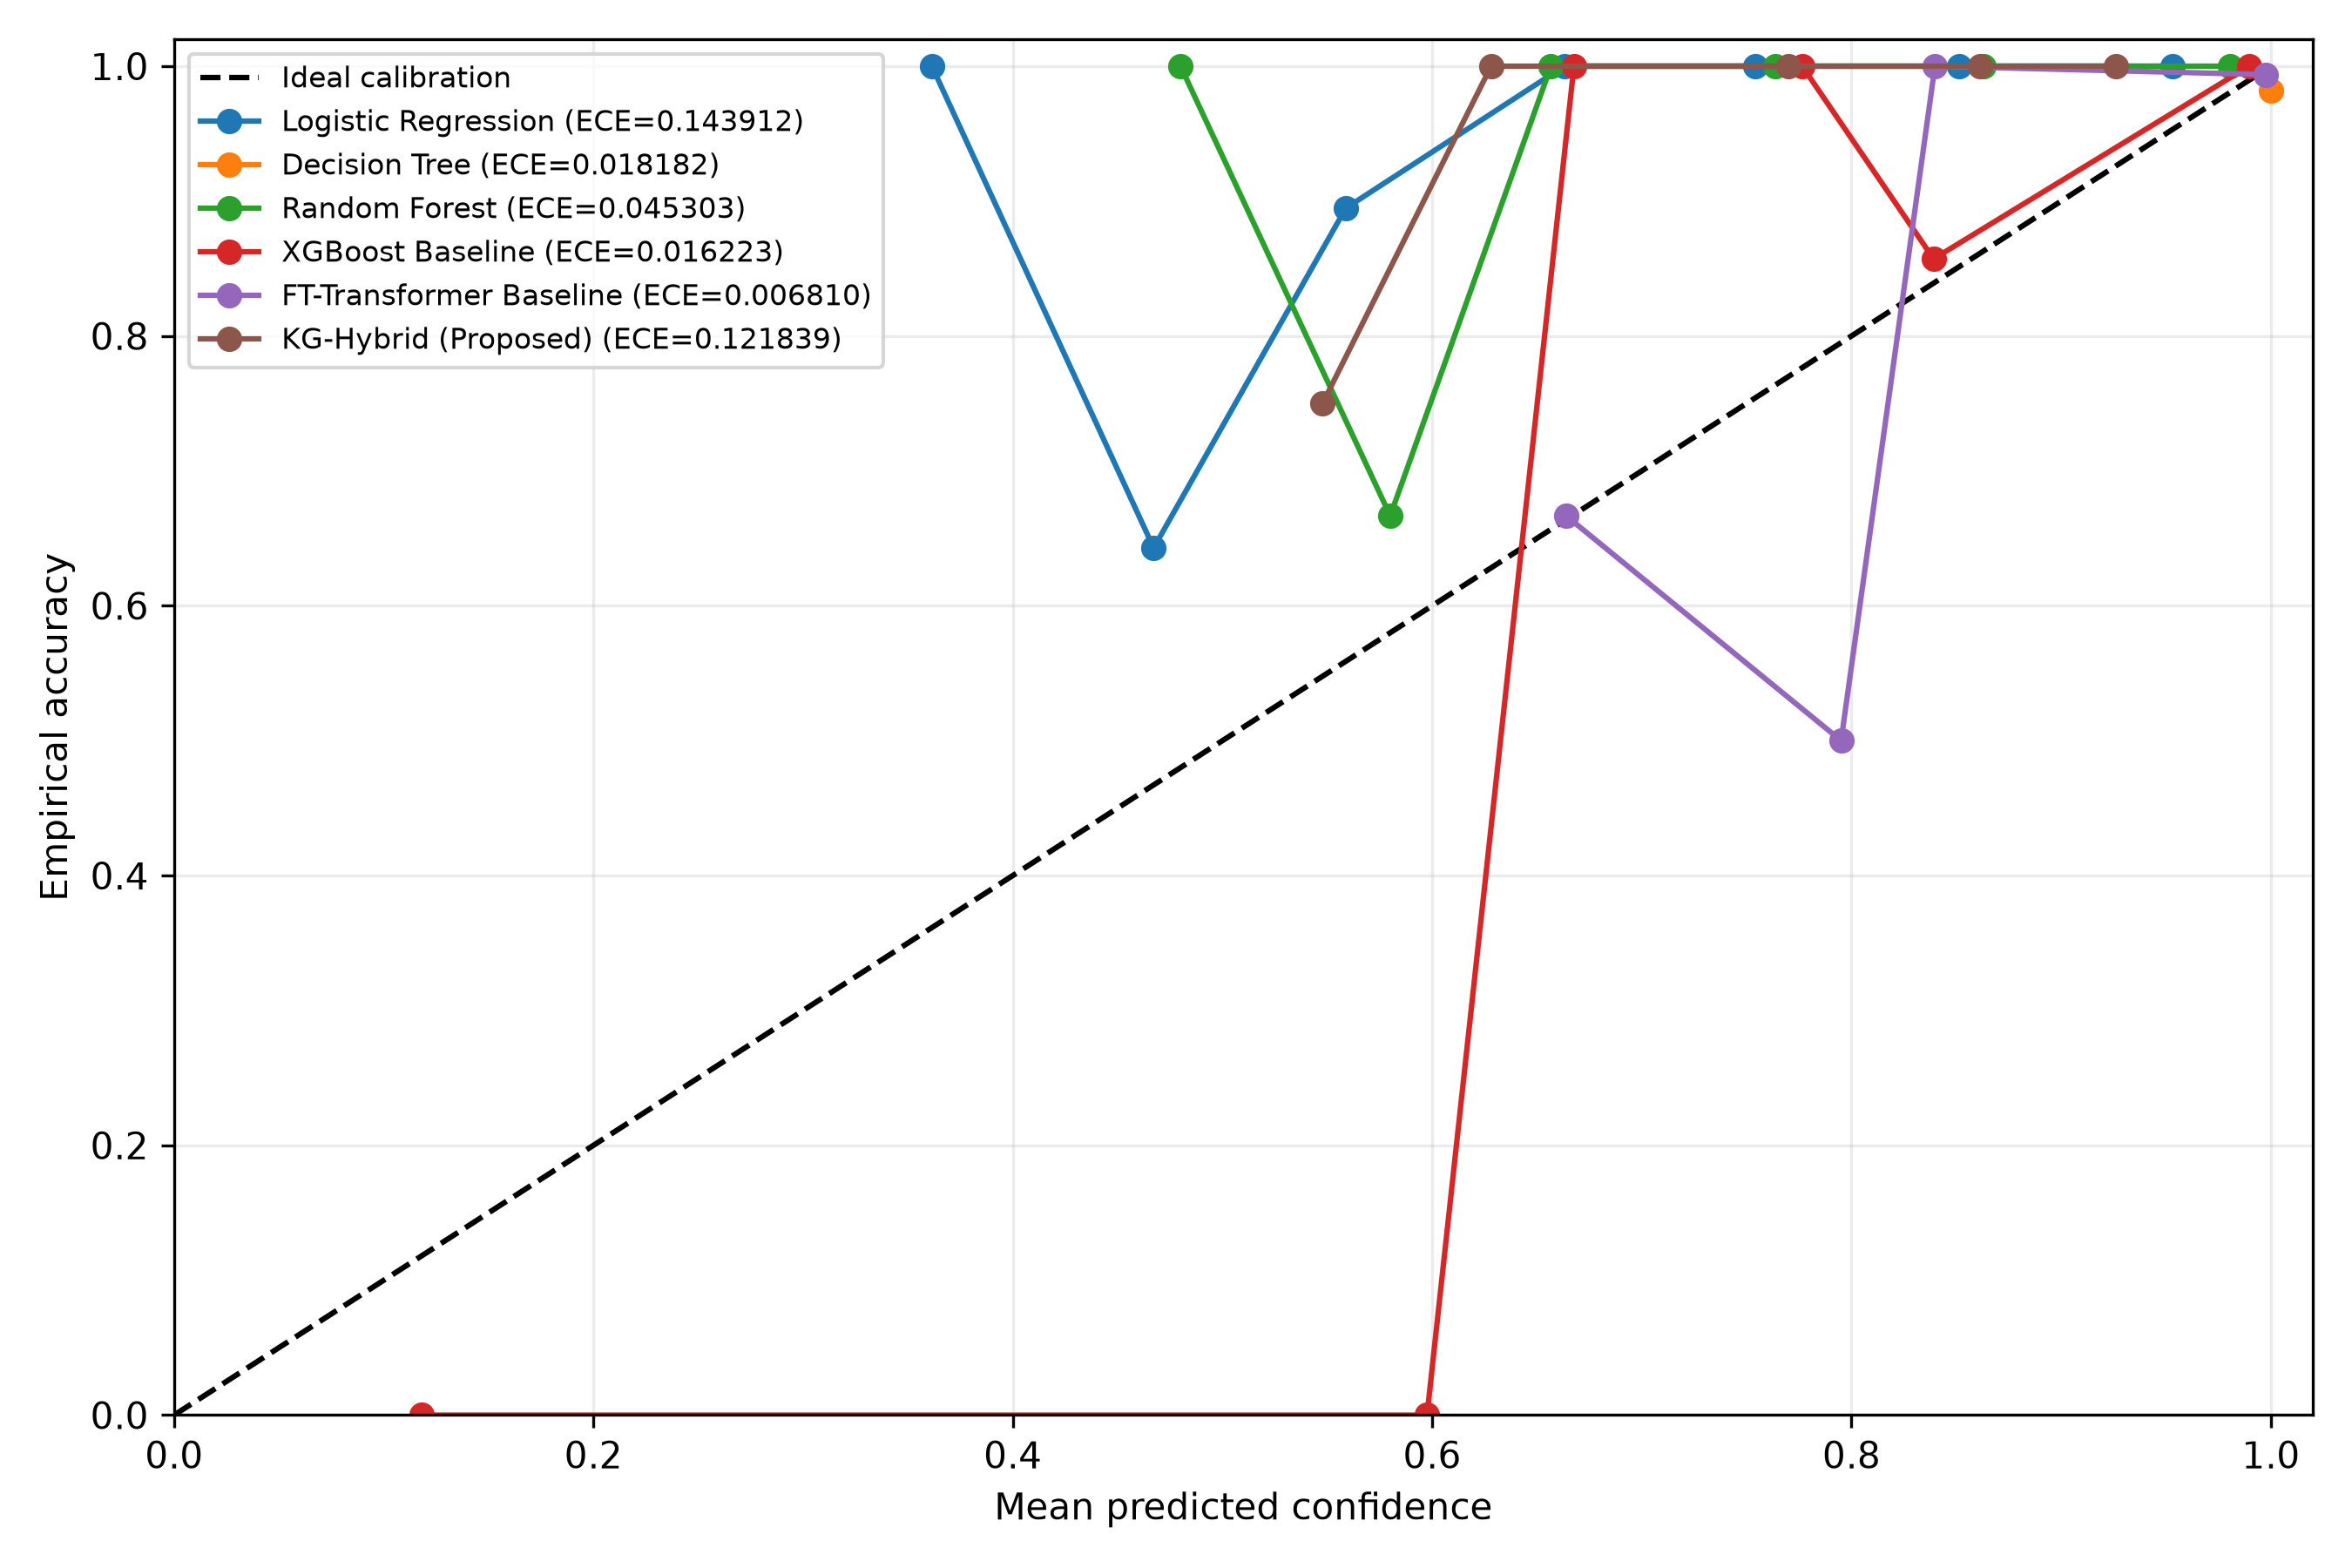
\includegraphics[width=\columnwidth]
{fig_f1_reliability_diagram.png}
\caption{Top-label reliability diagram for the saved-checkpoint
evaluation on 330 test records. Populated bins show empirical
accuracy against mean predicted confidence. The dashed diagonal
denotes ideal calibration.}
\label{fig:reliability}
\end{figure}

The historical checkpoint metadata does not establish that its
learned knowledge matrix was trained with the anchoring policy used
in the compact comparison. The difference between these probability
results cannot therefore be attributed to anchoring, compact
embeddings, or gating alone.

% --------------------------------------------------------------------
\subsection{Controlled Component Analysis}
% --------------------------------------------------------------------

The compact comparison separates the removal of knowledge context,
fixed versus anchored knowledge, and the addition of adaptive gating.
All variants use the same seed-specific partitions and controlled
training objective.

Adding the gate to the anchored-knowledge model leaves mean accuracy
unchanged at $99.4545\%$, while mean ECE decreases from
0.007033 to 0.004269. However, mean Brier score increases from
0.007597 to 0.008564, and mean NLL increases from
0.012481 to 0.015230. The gate therefore does not improve
every probability metric.

The no-knowledge hybrid exceeds the full model in mean accuracy by
approximately 0.1212 percentage points. The fixed-knowledge,
ungated variant also has slightly higher mean accuracy.
These results do not support a claim that the complete configuration
is uniformly preferable to its simpler alternatives.

The shuffled-knowledge variant obtains lower mean accuracy and
Macro-F1 than the full model. However, it uses fixed knowledge,
whereas the full model uses anchored trainable knowledge.
The comparison changes both profile alignment and knowledge policy;
it is not a pure one-factor test of agronomic profile alignment.

Exploratory statistical comparisons use paired tests on the five
seed-level differences: a paired $t$-test, equivalently a one-sample
$t$-test on paired differences, and a Wilcoxon signed-rank test.
Holm adjustment is applied across the 30 recorded
comparator--metric comparisons, separately for each test family.

For full-model ECE relative to XGBoost, the Holm-adjusted
$p$-values are 0.201748 for the paired $t$-test and 1.000000
for the Wilcoxon test. Neither establishes significance at
$\alpha=0.05$. Accuracy comparisons with XGBoost and the
no-knowledge hybrid likewise do not establish an advantage
for the full model.

Only five paired evaluations are available, and the seed-specific
partitions overlap. These tests have limited power and should not
be interpreted as comparisons across independent agricultural
populations. A nonsignificant result also does not establish
equivalence between models.

% --------------------------------------------------------------------
\subsection{Training Behavior and Knowledge Adaptation}
% --------------------------------------------------------------------

For the full compact configuration, the selected validation-NLL
checkpoint epochs are 8, 7, 14, 18, and 16 for seeds
42, 123, 2024, 3407, and 9999, respectively.
These values describe checkpoint selection within the
25-epoch budget, rather than independent evidence of generalization.

The fixed-knowledge variants preserve their initial matrices
without modification. For the full anchored configuration,
the mean absolute knowledge-matrix change, averaged across seeds,
is approximately $3.04\times10^{-4}$.
The largest absolute entry change observed across its five
checkpoints is approximately $2.57\times10^{-3}$.

These diagnostics confirm that the implemented anchor discourages
large deviations from the manually specified prior.
They do not validate the agronomic correctness of the initial
weights or establish a physical interpretation for the learned
attention scores. Anchoring is a soft penalty rather than a
hard interval constraint.

% --------------------------------------------------------------------
\subsection{Per-Class Classification Behavior}
% --------------------------------------------------------------------

Per-class analysis uses the 2,200 OOF predictions of the completed
noncompact CV experiment. KG-Hybrid correctly classifies
2,185 records and misclassifies 15 records.

Nine rice records are predicted as jute, and two jute records are
predicted as rice. The remaining errors comprise one jute record
predicted as coffee, one kidneybeans record predicted as pigeonpeas,
and two mothbeans records predicted as blackgram and lentil,
respectively.

Rice and jute have pooled OOF F1 scores of approximately
94.30\% and 94.17\%, respectively, below the aggregate
benchmark score. Their confusion identifies a limitation of the
evaluated classifier, but does not by itself establish an
agronomic explanation for the errors.

Fig.~\ref{fig:confusion} summarizes this complete OOF evaluation.
The matrix is not derived from the compact-model test partitions.

\begin{figure}[t]
\centering
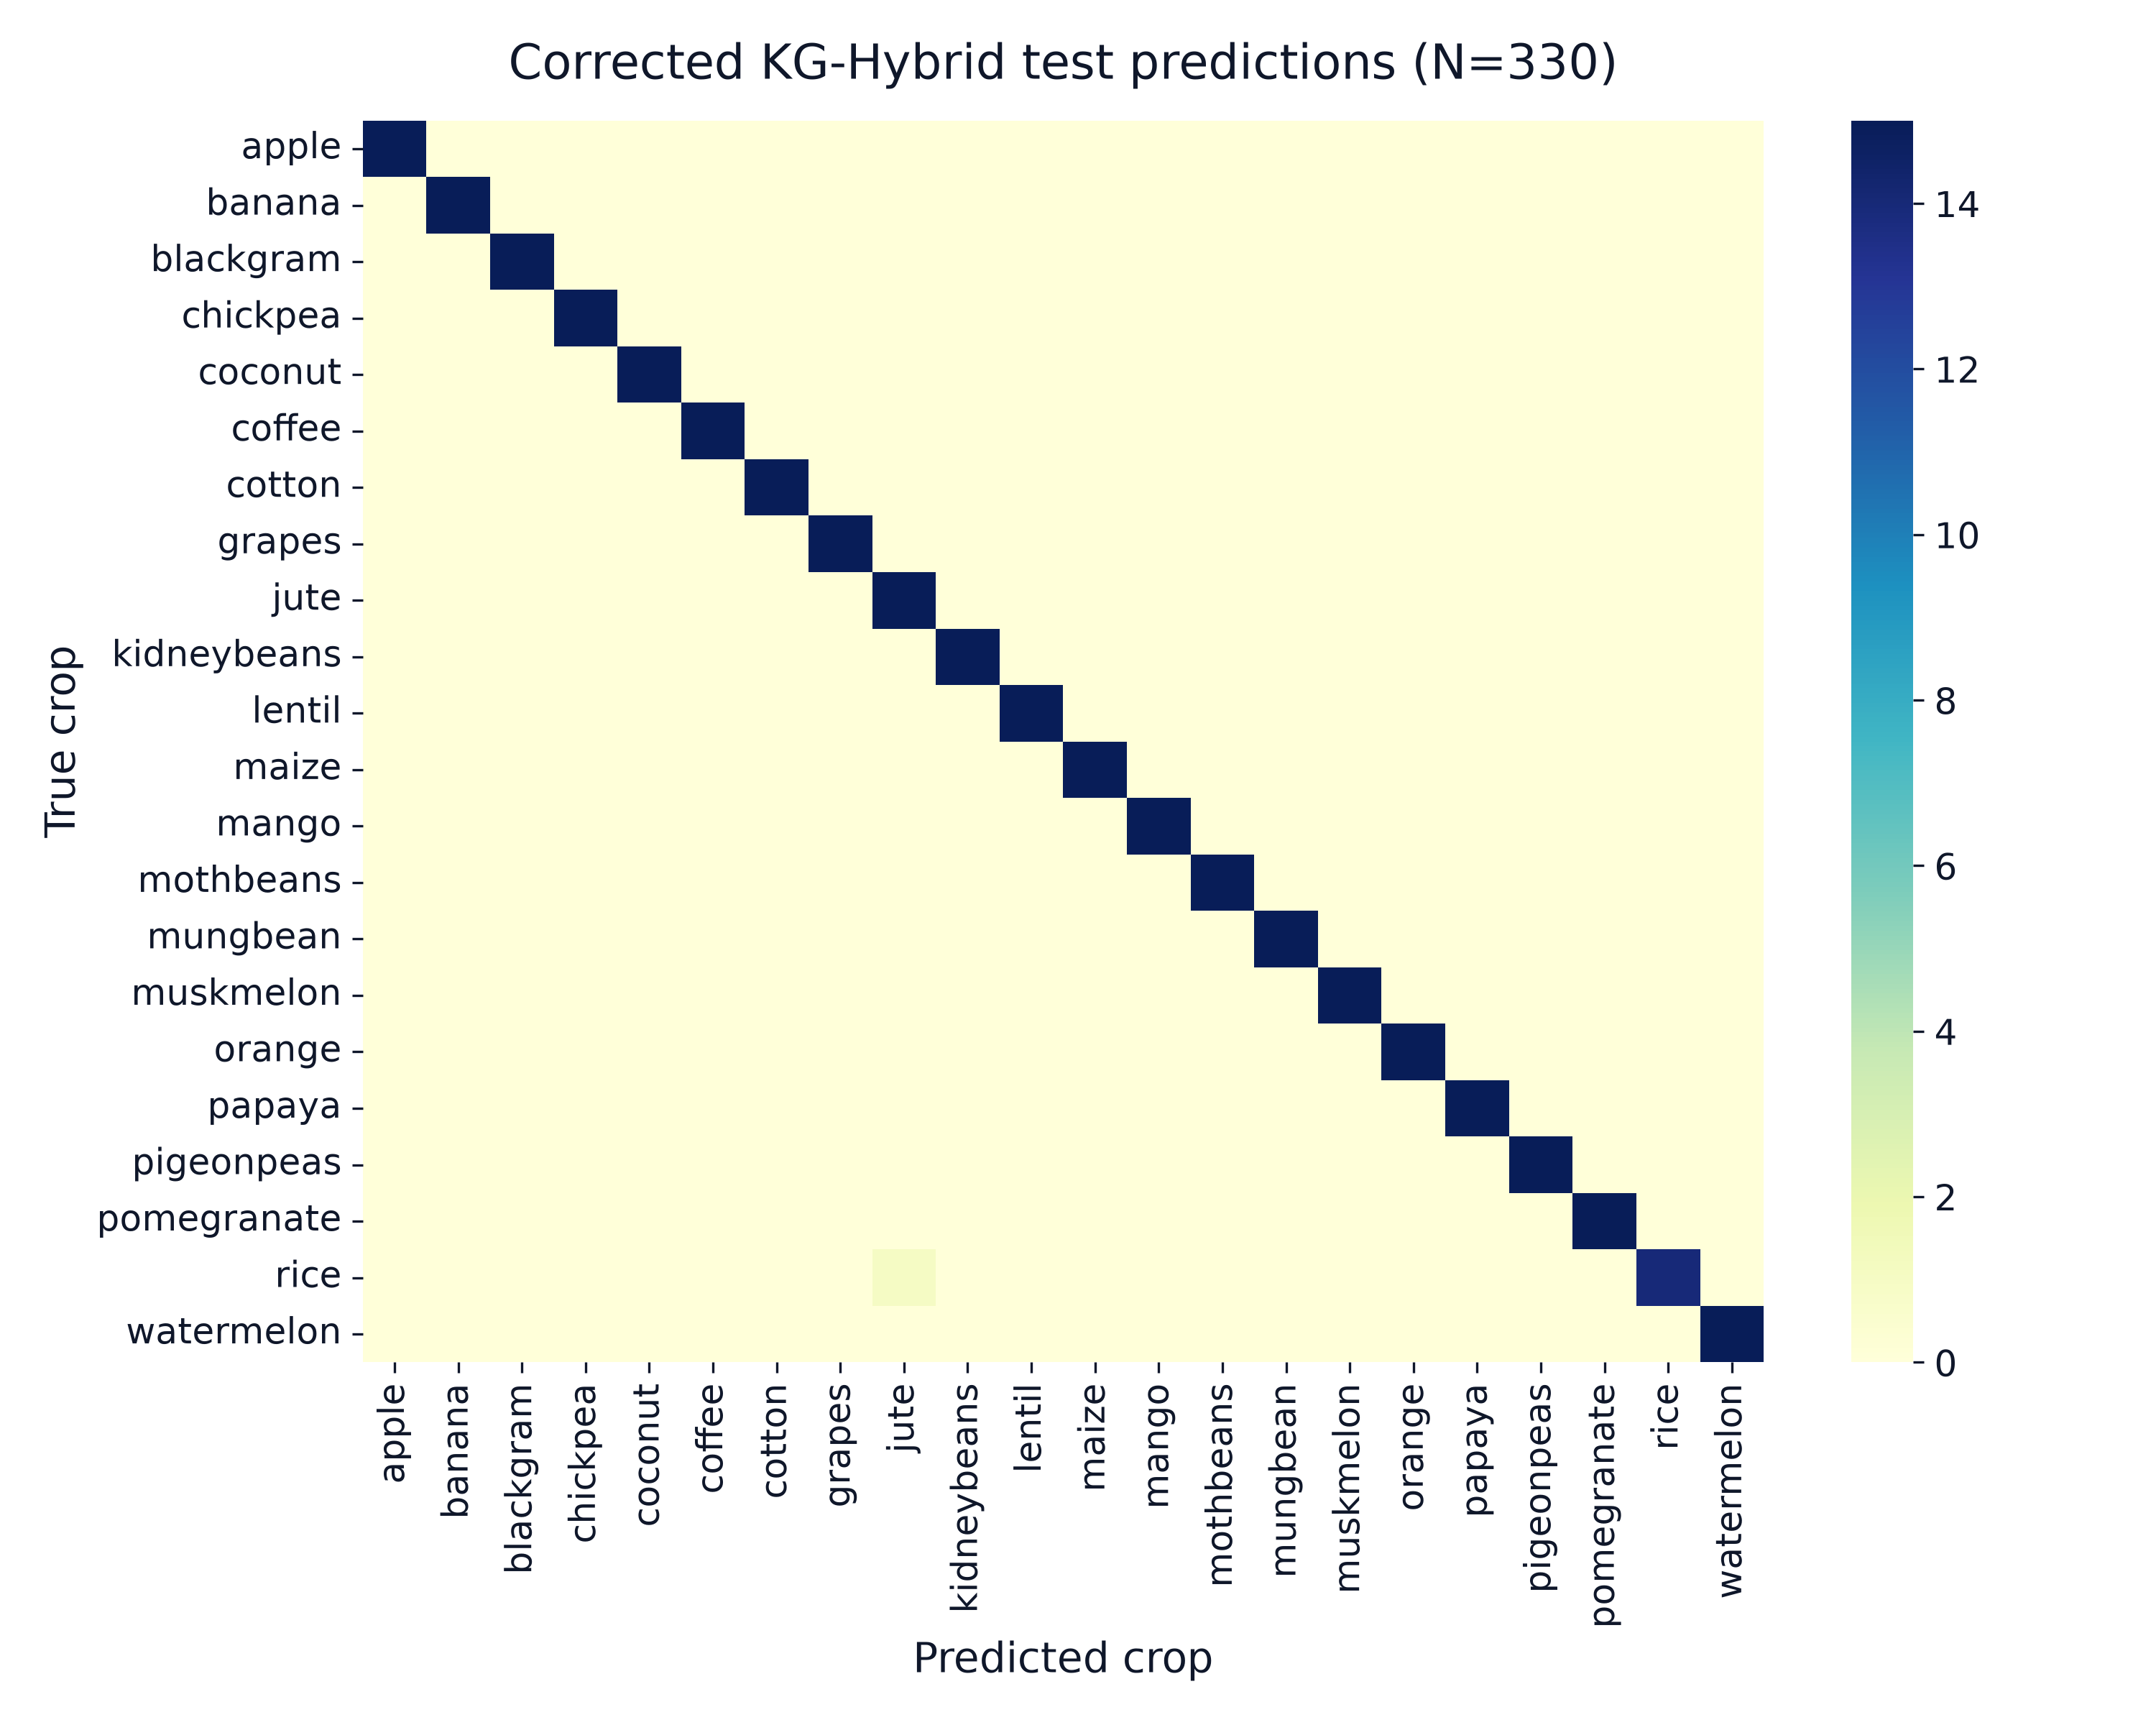
\includegraphics[width=\columnwidth]
{fig_f2_confusion_matrix_annotated.png}
\caption{Normalized KG-Hybrid confusion matrix computed from
2,200 OOF predictions in the completed noncompact five-fold
experiment. Rows denote true crop classes and columns denote
predicted classes. Each true class has support 100.}
\label{fig:confusion}
\end{figure}

% --------------------------------------------------------------------
\subsection{Exploratory Robustness Evidence}
% --------------------------------------------------------------------

Earlier saved robustness experiments examine incomplete inputs,
Gaussian perturbations, and feature scaling using noncompact
saved-model configurations. These experiments have not been
repeated for the compact models in
Table~\ref{tab:compact_comparison}. Their results characterize
the recorded earlier configurations only.

\subsubsection{Random Feature Masking}

The recorded masking experiment independently replaces each
standardized feature value with zero at probabilities
0.2, 0.4, and 0.6. Results average five perturbation trials.
Zero replacement corresponds to the training mean in standardized
coordinates; it is not the same protocol as representing missing
values with NaNs followed by KNN imputation.


\begin{figure}[t]
\centering
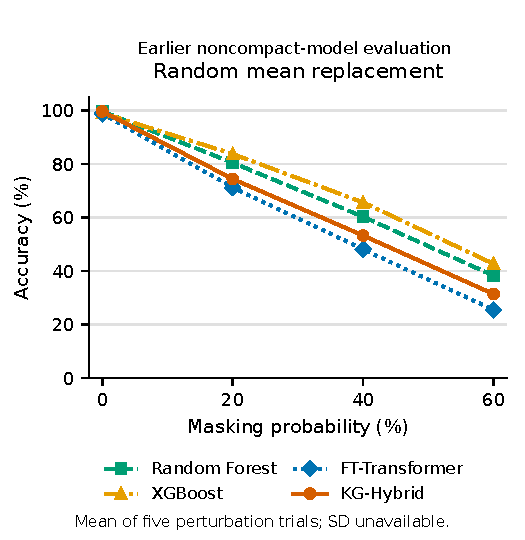
\includegraphics[width=\columnwidth]
{table_replacement_figures/table_x_feature_masking.pdf}
\caption{Earlier recorded zero-replacement experiment.
Points show mean accuracy over five perturbation trials.
Each standardized feature entry is independently replaced by
zero at the indicated probability. Trial-level standard deviations
are unavailable. These are not compact-model results.}
\label{fig:results_missing_features}
\end{figure}

All classifiers degrade as the replacement probability increases.
XGBoost has the highest recorded accuracy at each nonzero
masking level. KG-Hybrid exceeds FT-Transformer but does not
outperform the tree baselines under this protocol.

A separate earlier imputation comparison uses NaN masking and
imputers fitted on the standardized training data.
At 40\% masking, its recorded KG-Hybrid accuracy is
48.24\% with zero replacement and 81.33\% with
five-neighbor KNN imputation. The corresponding clean-model
accuracy is 97.88\%, identifying this as a different checkpoint
evaluation from Fig.~\ref{fig:results_missing_features}.
The imputation result is therefore interpreted only within
its own experiment.

\subsubsection{Gaussian Perturbations and Feature Scaling}

The Gaussian experiment adds independent noise to standardized
inputs and averages five trials at each noise level.
Thus, $\sigma$ denotes perturbation magnitude in standardized
feature coordinates, not a common physical sensor unit.

The feature-scaling experiment multiplies the standardized test
vectors by 1.5 while retaining their original labels.
This operation increases displacement from the training mean,
but does not ensure that every perturbed value lies outside the
training range. It is a synthetic stress test rather than
evaluation on an independently collected dataset.

\begin{figure}[t]
\centering
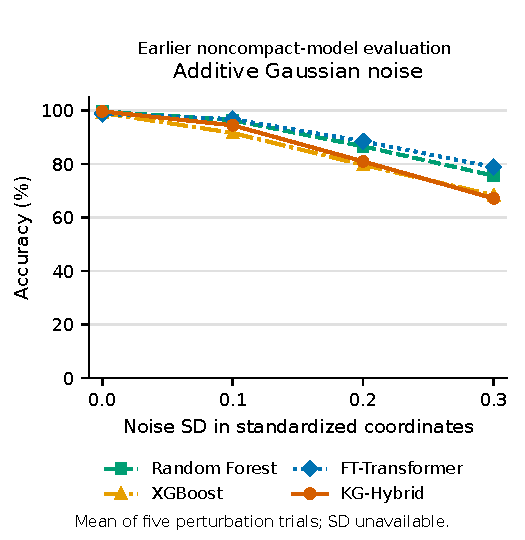
\includegraphics[width=\columnwidth]
{table_replacement_figures/table_xii_gaussian_noise.pdf}
\caption{Earlier recorded Gaussian-perturbation experiment.
Points show mean accuracy over five perturbation trials.
Noise magnitudes refer to standardized feature coordinates.
Trial-level standard deviations are unavailable.
These are not compact-model results.}
\label{fig:results_noise}
\end{figure}

\begin{figure}[t]
\centering
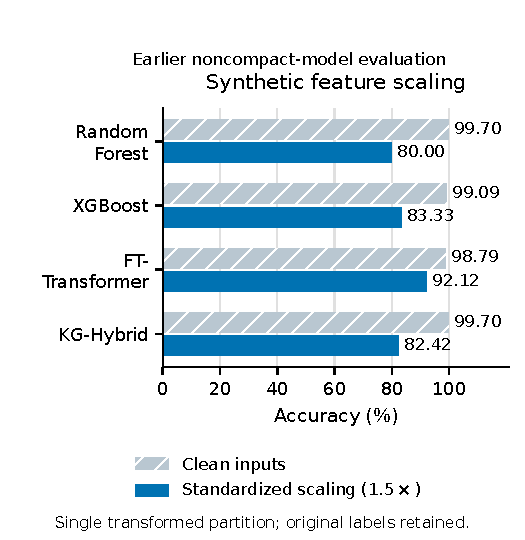
\includegraphics[width=\columnwidth]
{table_replacement_figures/table_xiii_feature_scaling.pdf}
\caption{Earlier recorded synthetic feature-scaling experiment.
Bars compare clean-input accuracy with accuracy after multiplying
standardized test vectors by $1.5\times$.
The transformed partition retains the original benchmark labels.
These are not compact-model results or external-dataset validation.}
\label{fig:results_scaling}
\end{figure}

FT-Transformer has the highest recorded accuracy under both
conditions in Figs.~\ref{fig:results_noise} and~\ref{fig:results_scaling}.
KG-Hybrid does not show a general robustness advantage.
The results further demonstrate that a model's clean-data ranking
need not persist under input perturbations.

These exploratory measurements do not establish robustness to
real sensor failures, seasonality, geographical transfer, or
changes in agricultural practice. In addition, retaining the
original crop labels after feature perturbation does not verify
that those labels remain agronomically appropriate.

% --------------------------------------------------------------------
\subsection{Confidence-Aware Routing}
% --------------------------------------------------------------------

Routing is evaluated separately using deterministic saved
XGBoost and corrected KG-Hybrid probabilities on 330 complete-input
test records. For threshold $\tau$, an input takes the
XGBoost fast path when its maximum XGBoost class probability
is at least $\tau$; otherwise, the corrected hybrid supplies
the prediction.

In the production policy, inputs requiring imputation are
ineligible for the fast path. The present audit contains only
complete inputs and does not measure the missing-input fallback.

\begin{table}[t]
\centering
\caption{Deterministic Saved-Checkpoint Routing Audit on
330 Complete-Input Records. Coverage Denotes XGBoost Exits.
No Latency or MC-Dropout Measurement Is Included.}
\label{tab:routing}
\small
\begin{tabular}{crrrr}
\hline
$\tau$ & XGB exits & Hybrid & Coverage (\%) & Accuracy (\%) \\
\hline
0.50 & 329 & 1   & 99.70 & 99.39 \\
0.70 & 325 & 5   & 98.48 & 99.70 \\
0.80 & 324 & 6   & 98.18 & 99.70 \\
0.85 & 320 & 10  & 96.97 & 99.70 \\
0.90 & 317 & 13  & 96.06 & 99.70 \\
0.95 & 310 & 20  & 93.94 & 99.70 \\
0.99 & 246 & 84  & 74.55 & 99.70 \\
1.00 & 0   & 330 & 0.00  & 99.70 \\
\hline
\end{tabular}
\end{table}

At $\tau=0.90$, 317 records take the XGBoost route and
13 use the hybrid, corresponding to 96.06\% fast-path
coverage. All 317 fast-path predictions are correct.
The hybrid correctly classifies 12 of the 13 fallback records,
giving overall cascade accuracy $329/330=99.70\%$.

Direct XGBoost accuracy is $327/330=99.09\%$, while
direct corrected-hybrid accuracy is $329/330=99.70\%$.
Fast-path predictions are XGBoost predictions and should not
be attributed to the knowledge-guided neural pathway.

The threshold 0.90 is an evaluated operating point, not a
universally optimal threshold or a guarantee of correctness
at 90\% confidence. Threshold results on this test set are
descriptive and do not replace validation-based threshold
selection.

Fig.~\ref{fig:risk_coverage} depicts a different selective-prediction
analysis: direct hybrid predictions are ordered by hybrid confidence,
and error is calculated among the retained predictions.
Its coverage is therefore not the XGBoost exit fraction in
Table~\ref{tab:routing}.

\begin{figure}[t]
\centering
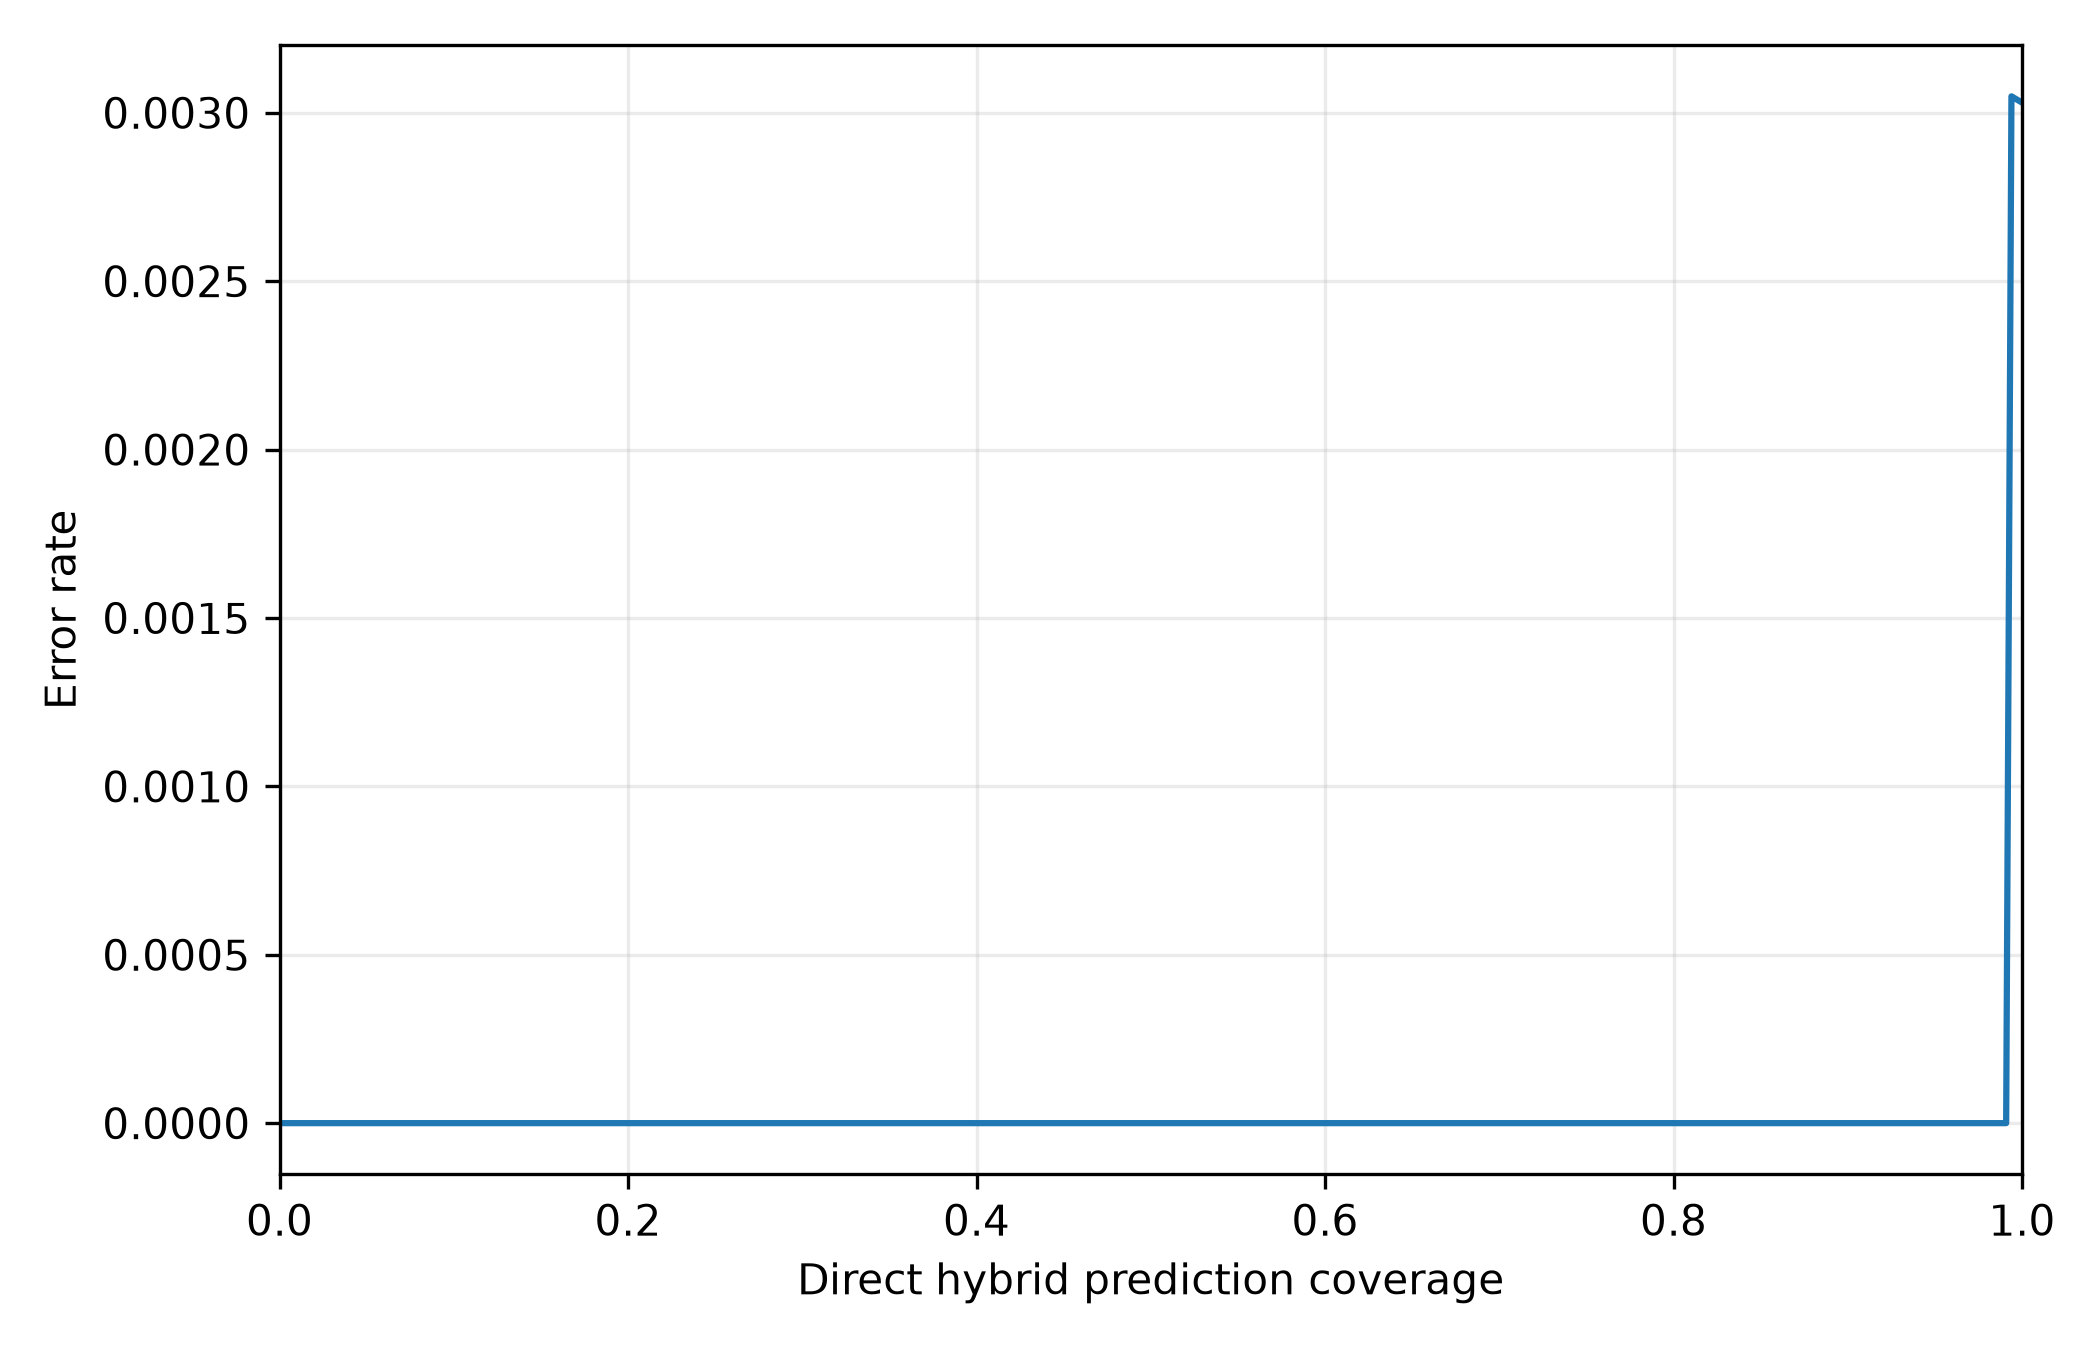
\includegraphics[width=\columnwidth]
{fig_f4_risk_coverage.png}
\caption{Risk--coverage curve for direct corrected-hybrid
predictions on the designated test partition. Coverage is the
fraction retained after ordering predictions by hybrid confidence;
risk is the error rate among retained predictions.
This is not a cascade-routing latency curve.}
\label{fig:risk_coverage}
\end{figure}

The deterministic audit excludes MC-Dropout inference,
imputation cost, and execution timing. Consequently, its
coverage values alone do not establish an end-to-end
latency reduction.

% --------------------------------------------------------------------
\subsection{Model Complexity and Computational Scope}
% --------------------------------------------------------------------

The compact representation allocates embeddings only to actual
terminal nodes of the seed-specific fitted booster, with
tree-specific identities. All terminal nodes are included,
including those not visited by training records.

For the full compact model, the vocabulary sizes range from
11,055 to 11,235 across the five seeds. The mean vocabulary
size is 11,144. At embedding dimension 128, this produces
a mean of 1,426,432 embedding-table parameters.

Fig.~\ref{fig:results_parameters} reports registered neural
parameter counts. These counts include parameters marked as
trainable in the model object; they are not counts of floating-point
operations or parameters necessarily updated by the hybrid objective.

\begin{figure*}[t]
\centering
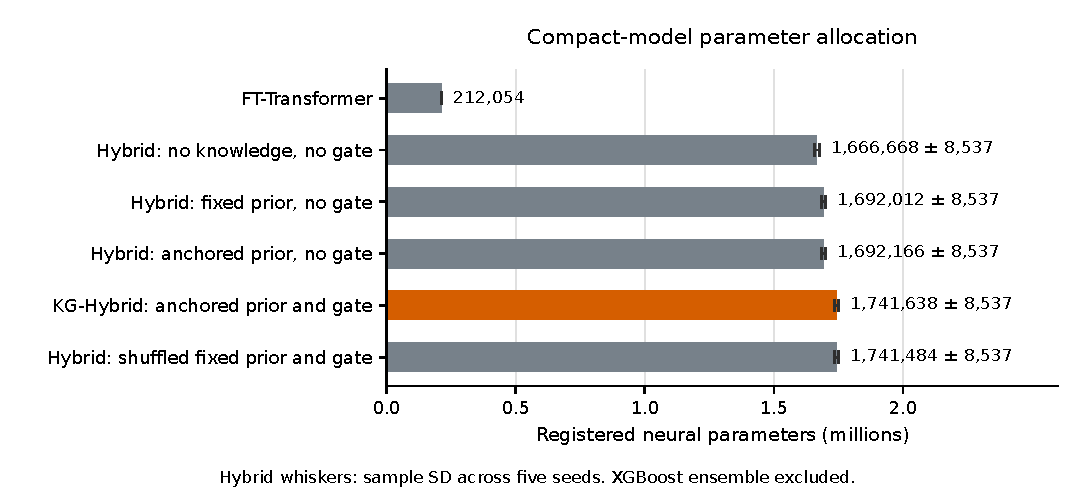
\includegraphics[width=\textwidth]
{table_replacement_figures/table_ix_registered_parameters.pdf}
\caption{Registered neural parameter counts in the compact
comparison. Hybrid bars show mean counts and whiskers show
sample standard deviations across five seeds.
The FT-Transformer count is constant across runs.
Counts include the retained standalone FT classification head,
which is bypassed by hybrid prediction.
The separately stored XGBoost ensemble is excluded.}
\label{fig:results_parameters}
\end{figure*}

The full hybrid's registered count includes the
11,158-parameter standalone FT classification head.
That head is bypassed by the fused prediction path.
Excluding it, the mean active fused-path parameter count
is 1,730,480, comprising the leaf embedder,
FT feature backbone, knowledge-guided fusion module,
and hybrid prediction head.

The external XGBoost ensemble is stored separately and contains
4,400 class-specific trees. Tree counts, node counts, serialized
size, and neural parameter counts are distinct complexity
measures and are not combined into a single parameter total.

A reconciled end-to-end latency benchmark has not been established
for the compact models. Timings obtained from earlier wrappers,
noncompact checkpoints, different batching conditions, or
MC-Dropout settings are therefore not reported as compact-model
latencies. The current evidence supports reduced embedding
allocation, but not a hardware-independent speedup, memory bound,
or edge-deployment claim. It is concluded that the 
 completed noncompact CV experiment yields
$99.32\pm0.28\%$ Macro-F1 for KG-Hybrid, with XGBoost
achieving the highest mean classification scores.
In the compact controlled comparison, the full model obtains
$99.45\pm0.25\%$ accuracy and
$99.46\pm0.25\%$ Macro-F1.
Simpler configurations remain competitive and, in some metrics,
perform better.

The compact full model has the lowest mean ECE, but its improvement
over XGBoost is not significant under the recorded Holm-adjusted
paired comparisons. The corrected saved noncompact checkpoint,
evaluated separately, exhibits substantially weaker calibration
despite high accuracy. These findings make probability reliability
a configuration- and protocol-dependent result.

